\section{Aufbau und Durchführung} % (fold)
\label{sec:versuchsaufbau}

	\subsection{Röntgenquelle} % (fold)
	\label{sub:rntgenquelle}
		
		Als Quelle der Röntgenstrahlung fungiert, wie unter Abschnitt \ref{ssub:rntgenbremsstrahlung} beschrieben, eine Röntgenröhre.
		Der konkrete Aufbau dieser ist in Abbildung \ref{apperat} zu sehen.
		In der Mitte der Konstruktion ist ein Würfel zu sehen, der die Röhre beinhaltet.
		Rechts der Röhre befindet sich ein Schlitten, auf dem die Kamera positioniert wird. 
		Die entstehende Strahlung verlässt den Würfel durch die rechte Fläche und dringt direkt durch eine Blende in die Kamera ein, um den Strahlenschutz zu gewährleisten.
		Für die Messung mit der Kupfer-Anode wird zwischen Kamera und Röhre noch ein passender Nickel-Filter befestigt.
		Wie in den Grundlagen beschrieben, ermöglicht dies näherungsweise die Verwendung der reinen $K_\alpha$-Linie von Kupfer, welche bei ungefähr $1.5425\unit{\AA}$ liegt.
		Der dahinter liegende Spiegel leitet das Licht des Fluoreszenzschirms der Kamera um, sodass während des Betriebs überprüft werden kann, ob Strahlung durch die Kamera läuft.
		Die Röhre wird mit einer Gleichspannung von $35 \unit{kV}$ und einem Strom von circa $ 10 \unit{mA} $ betrieben.

		\begin{figure}[htb]
			\centering
			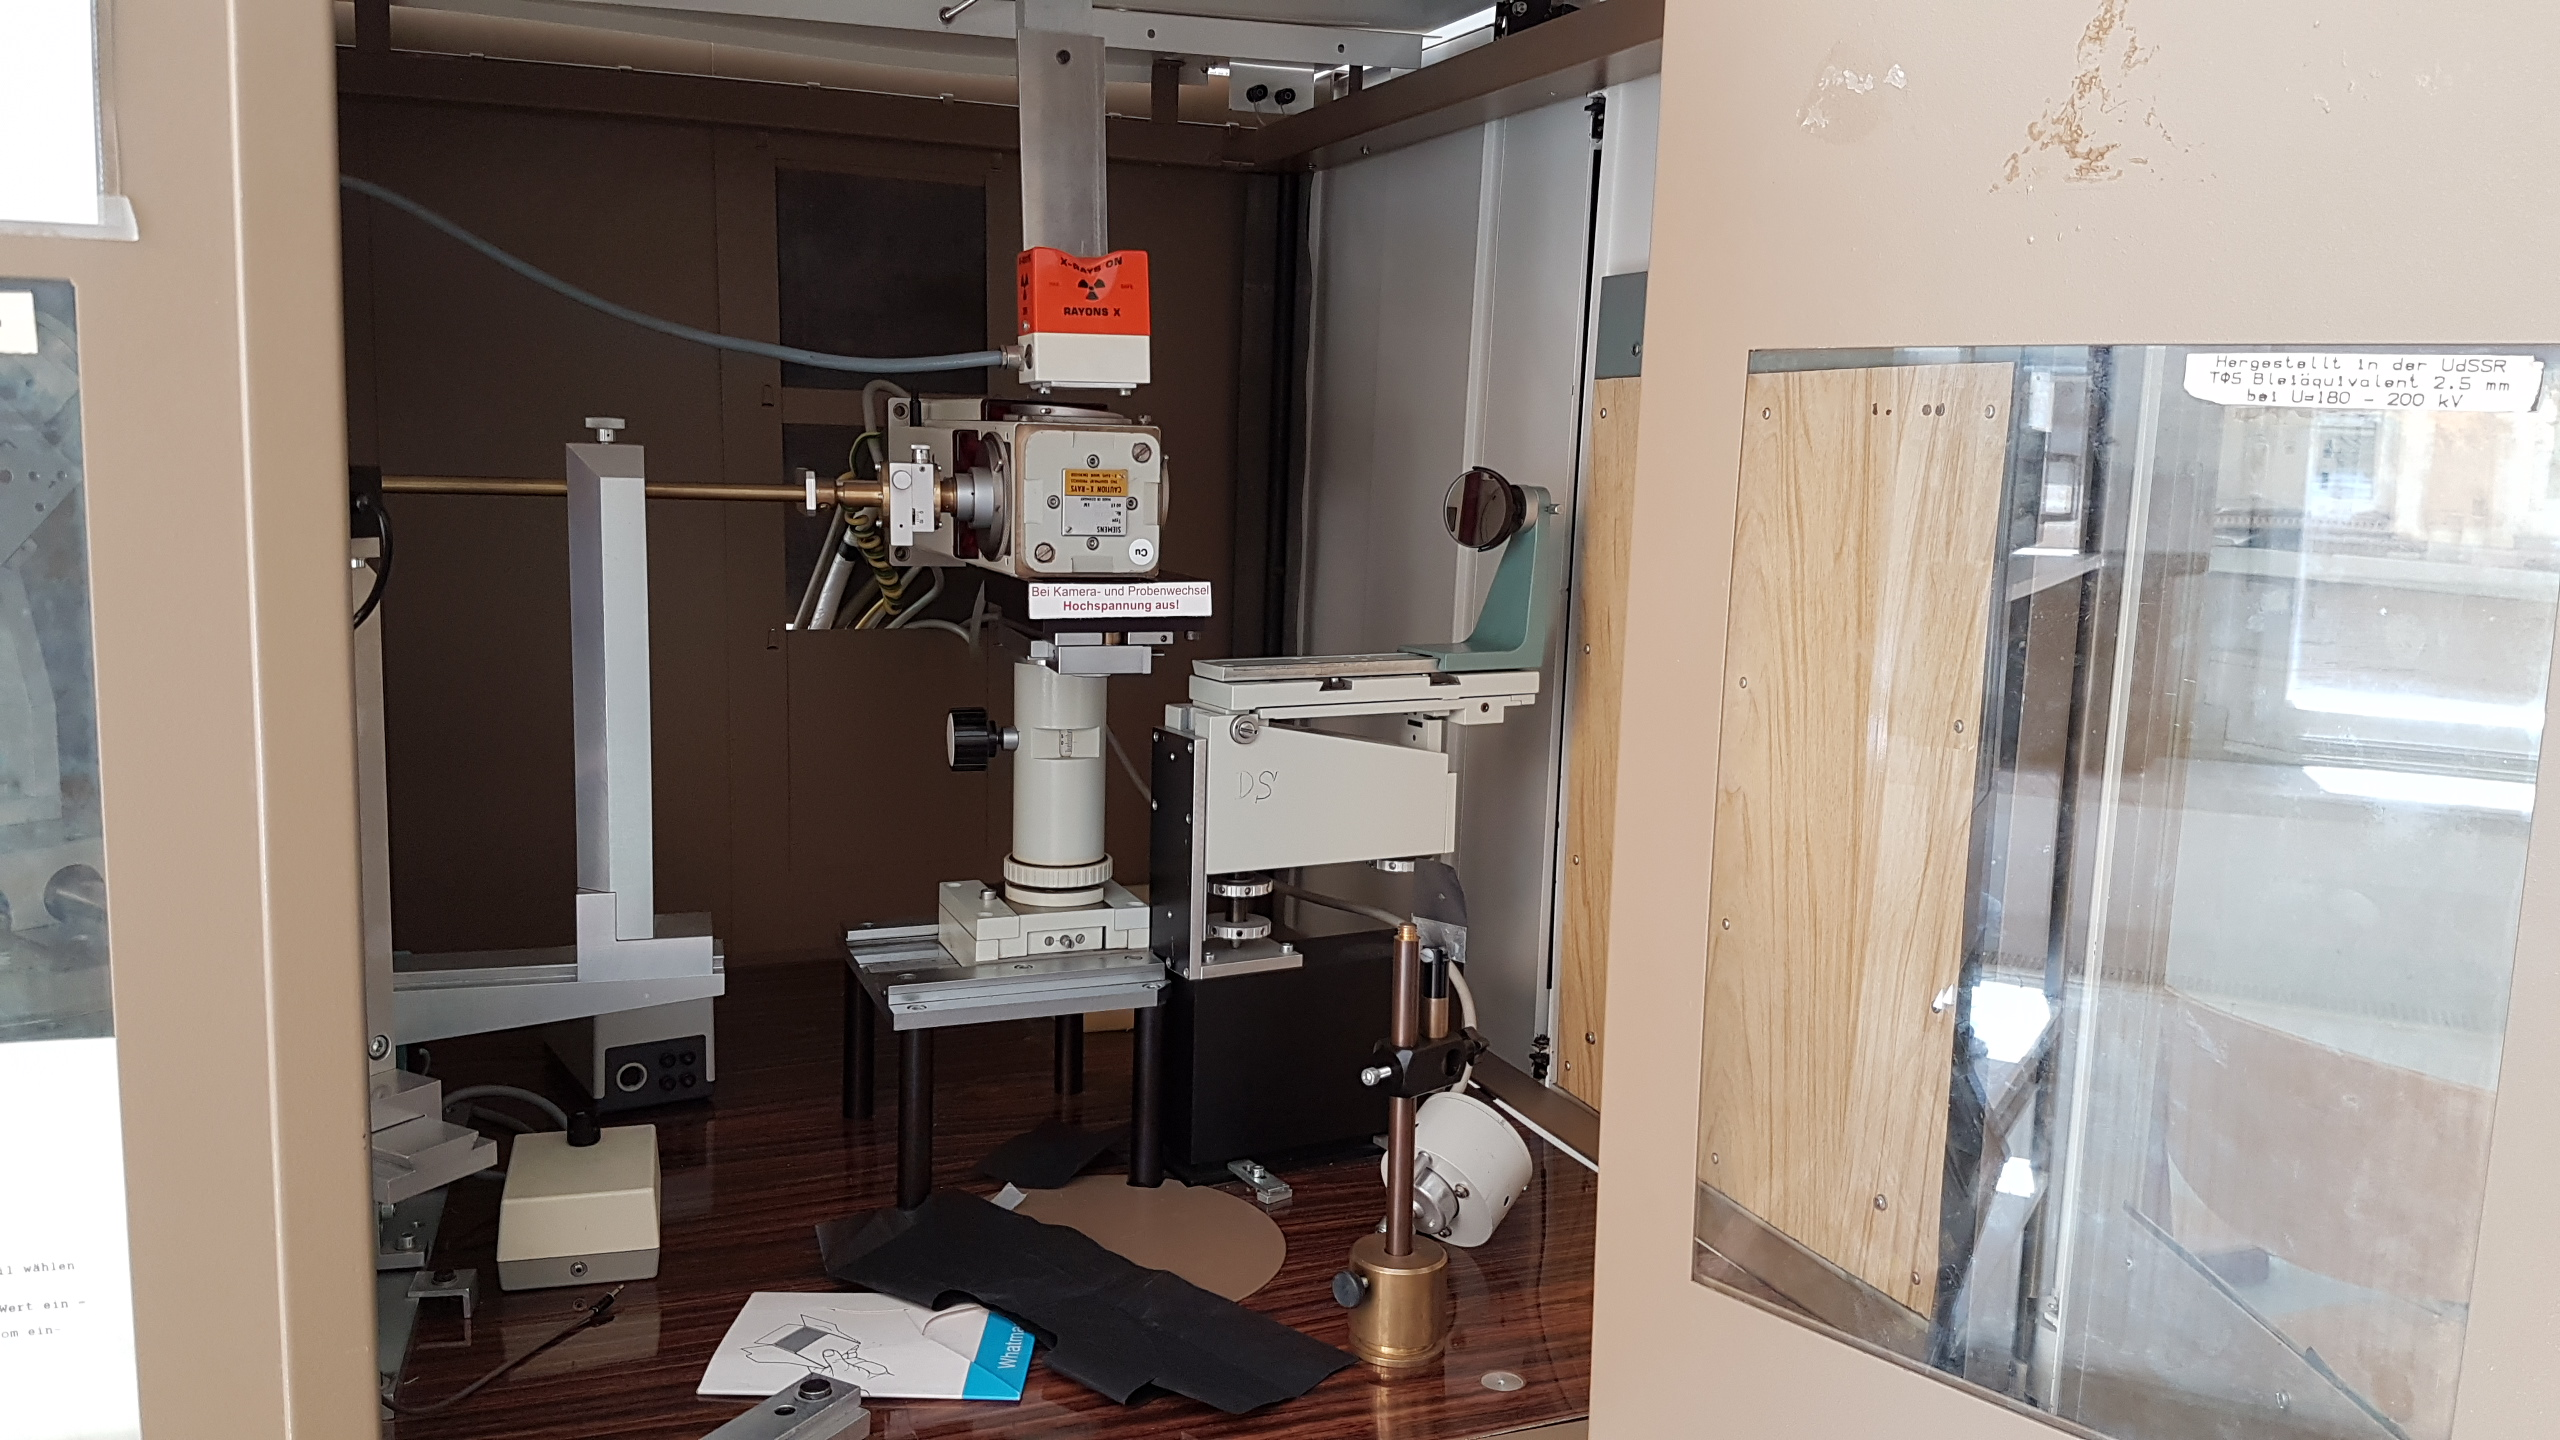
\includegraphics[scale = 0.12]{images/maschine.jpg}
			\caption{Röntgenapperat mit Röhre, Metallfiltern, Kameraführung und Umlenkspiegel}
			\label{apperat}
		\end{figure}

	% subsection röntgenquelle (end)

	\subsection{Die Kamera} % (fold)
	\label{sub:die_kamera}
		
		Der zu untersuchende Kristall befindet sich auf einer drehbaren Achse gelagert in der Mitte der Kamera, welche in Abbildung \ref{fig:kamera} zu sehen ist.
		Der Primärstrahl dringt durch die vordere Öffnung ein, in der die Blende eingebracht werden kann, um den Strahl möglichst klein und kollimiert auf den Kristall treffen zu lassen.
		Auf der Rückseite befindet sich der Fluoreszenzschirm vor einem Bleiglasfenster.
		Die Schwalbenschwanzführung ermöglicht das Positionieren der Kamera vor der Röhre.
		Der Zahnradkranz am Deckel steuert die Drehung der Achse und lässt sich über den Motor bewegen, der in Abbildung \ref{apperat} unten rechts zu sehen ist.
		An den Innenwänden der Kamera wird dann der Film aufgespannt und fixiert.
		Der Radius der Kamera beträgt $57.5\unit{mm}$.

		\begin{figure}[htb]
			\centering
			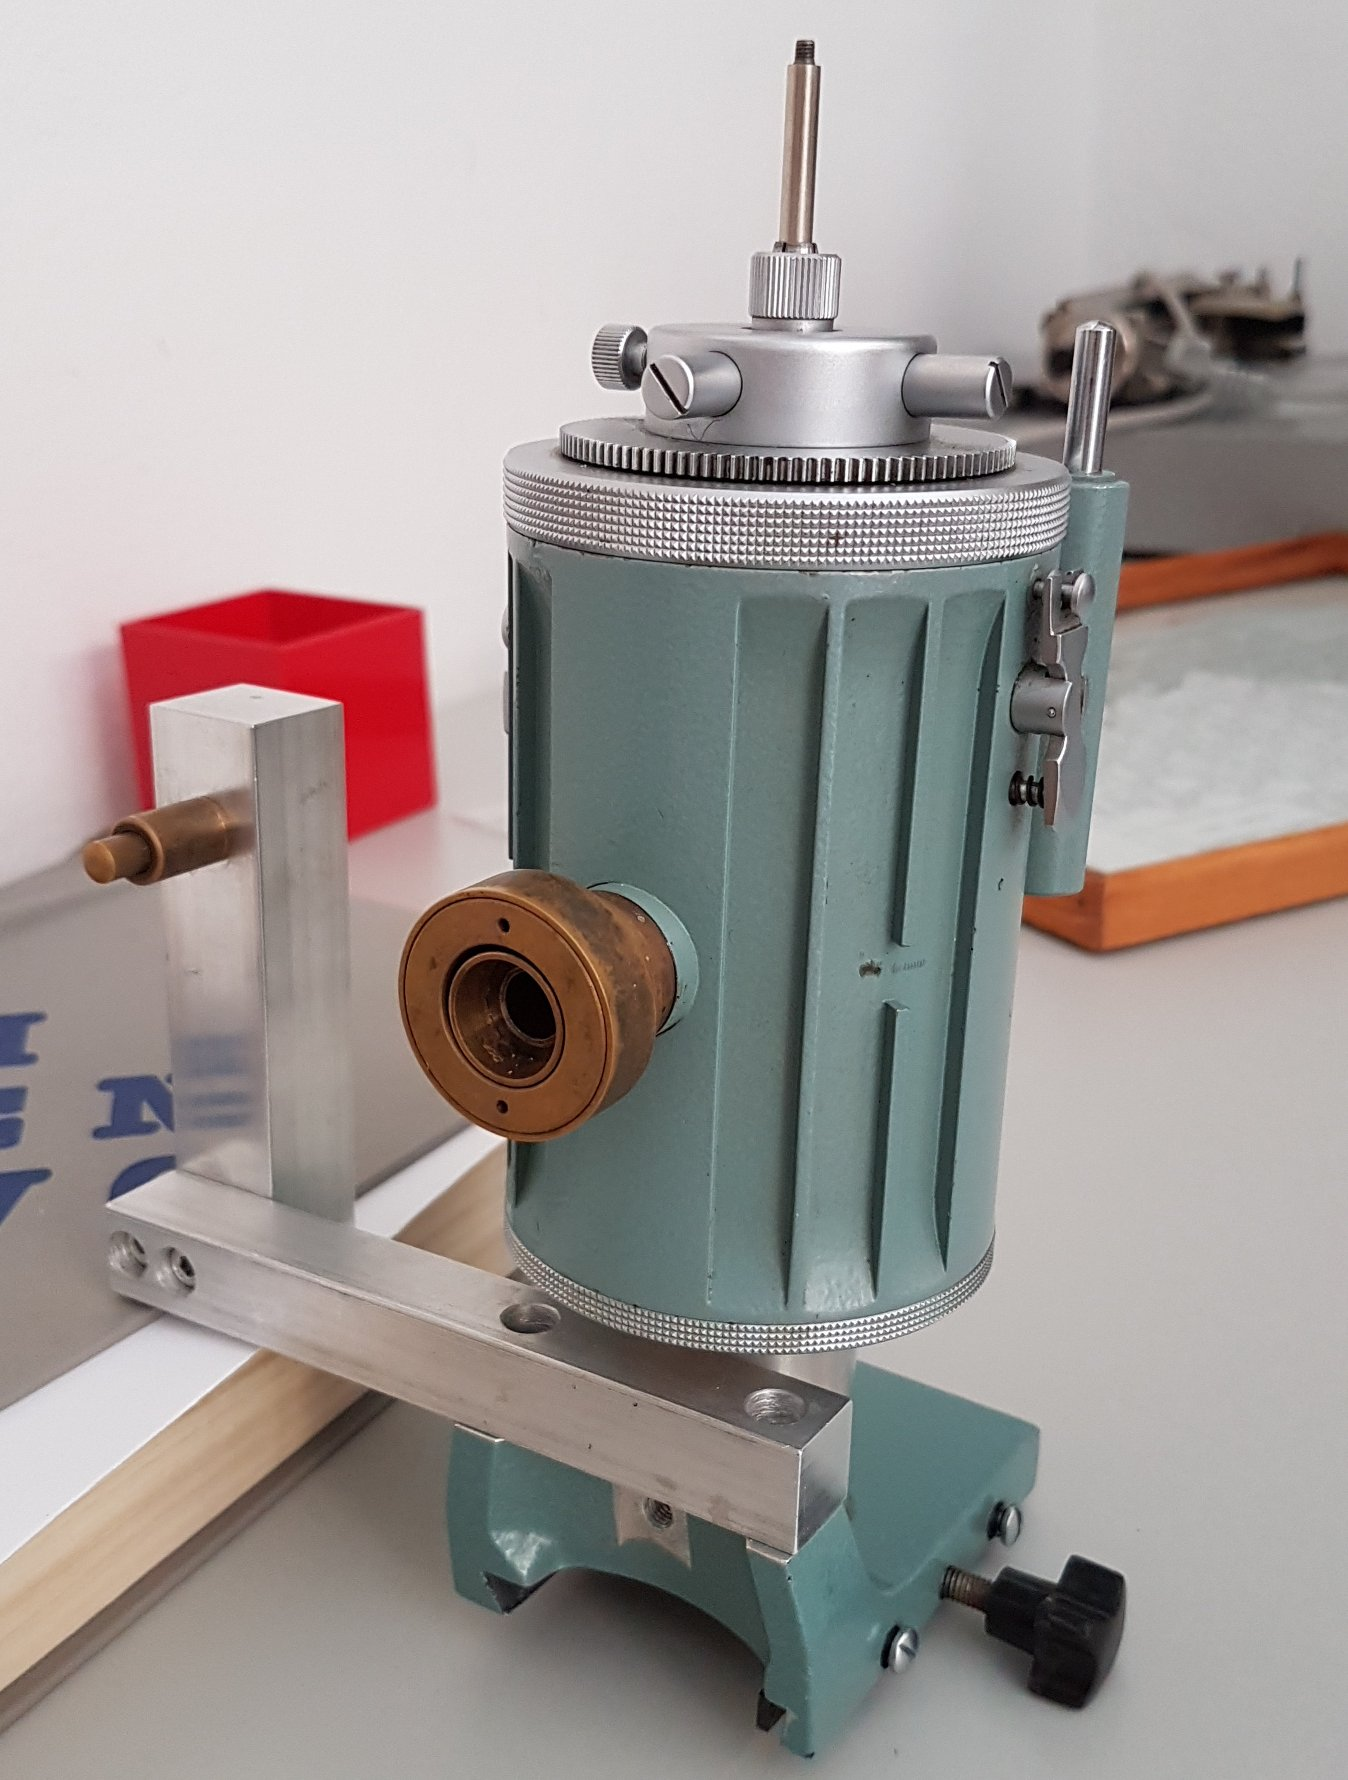
\includegraphics[scale = 0.2]{images/kamera-2.jpg}
			\caption{Aufnahmekamera mit drehbarer Achse, Zahnradkranz und Primärstrahleintritt}
			\label{fig:kamera}
		\end{figure}

	% subsection die_kamera (end)

	\subsection{Justierung der Kristallachse} % (fold)
	\label{sub:justierung_der_kristallachse}

		Zunächst wird ein kleinerer Kristall, wie er in Abbildung \ref{fig:kristall} zu sehen ist, mit einem Meißel von einem größeren Block abgespalten.
		Dabei brechen die Kristalle bevorzugt entlang einer niedrig indizierten Achse, also meist $(100)$, $(001)$ oder $(010)$.
		Anschließend kann man den Splitter mittels Klebewachs an der Drehachse befestigen.
		Die genaue Ausrichtung erfolgt am Goniometer, dargestellt in Abbildung \ref{fig gonio}.
		Hier wird ein kleiner Leuchtfleck auf eine der Seitenflächen des Kristalls projiziert.
		Der Kristall wird anschließend über zwei Stellschrauben so lange verkippt, bis die Reflexion des Flecks immer in der gleichen Ebene erfolgt.

		\begin{figure}[htb]
			\centering
			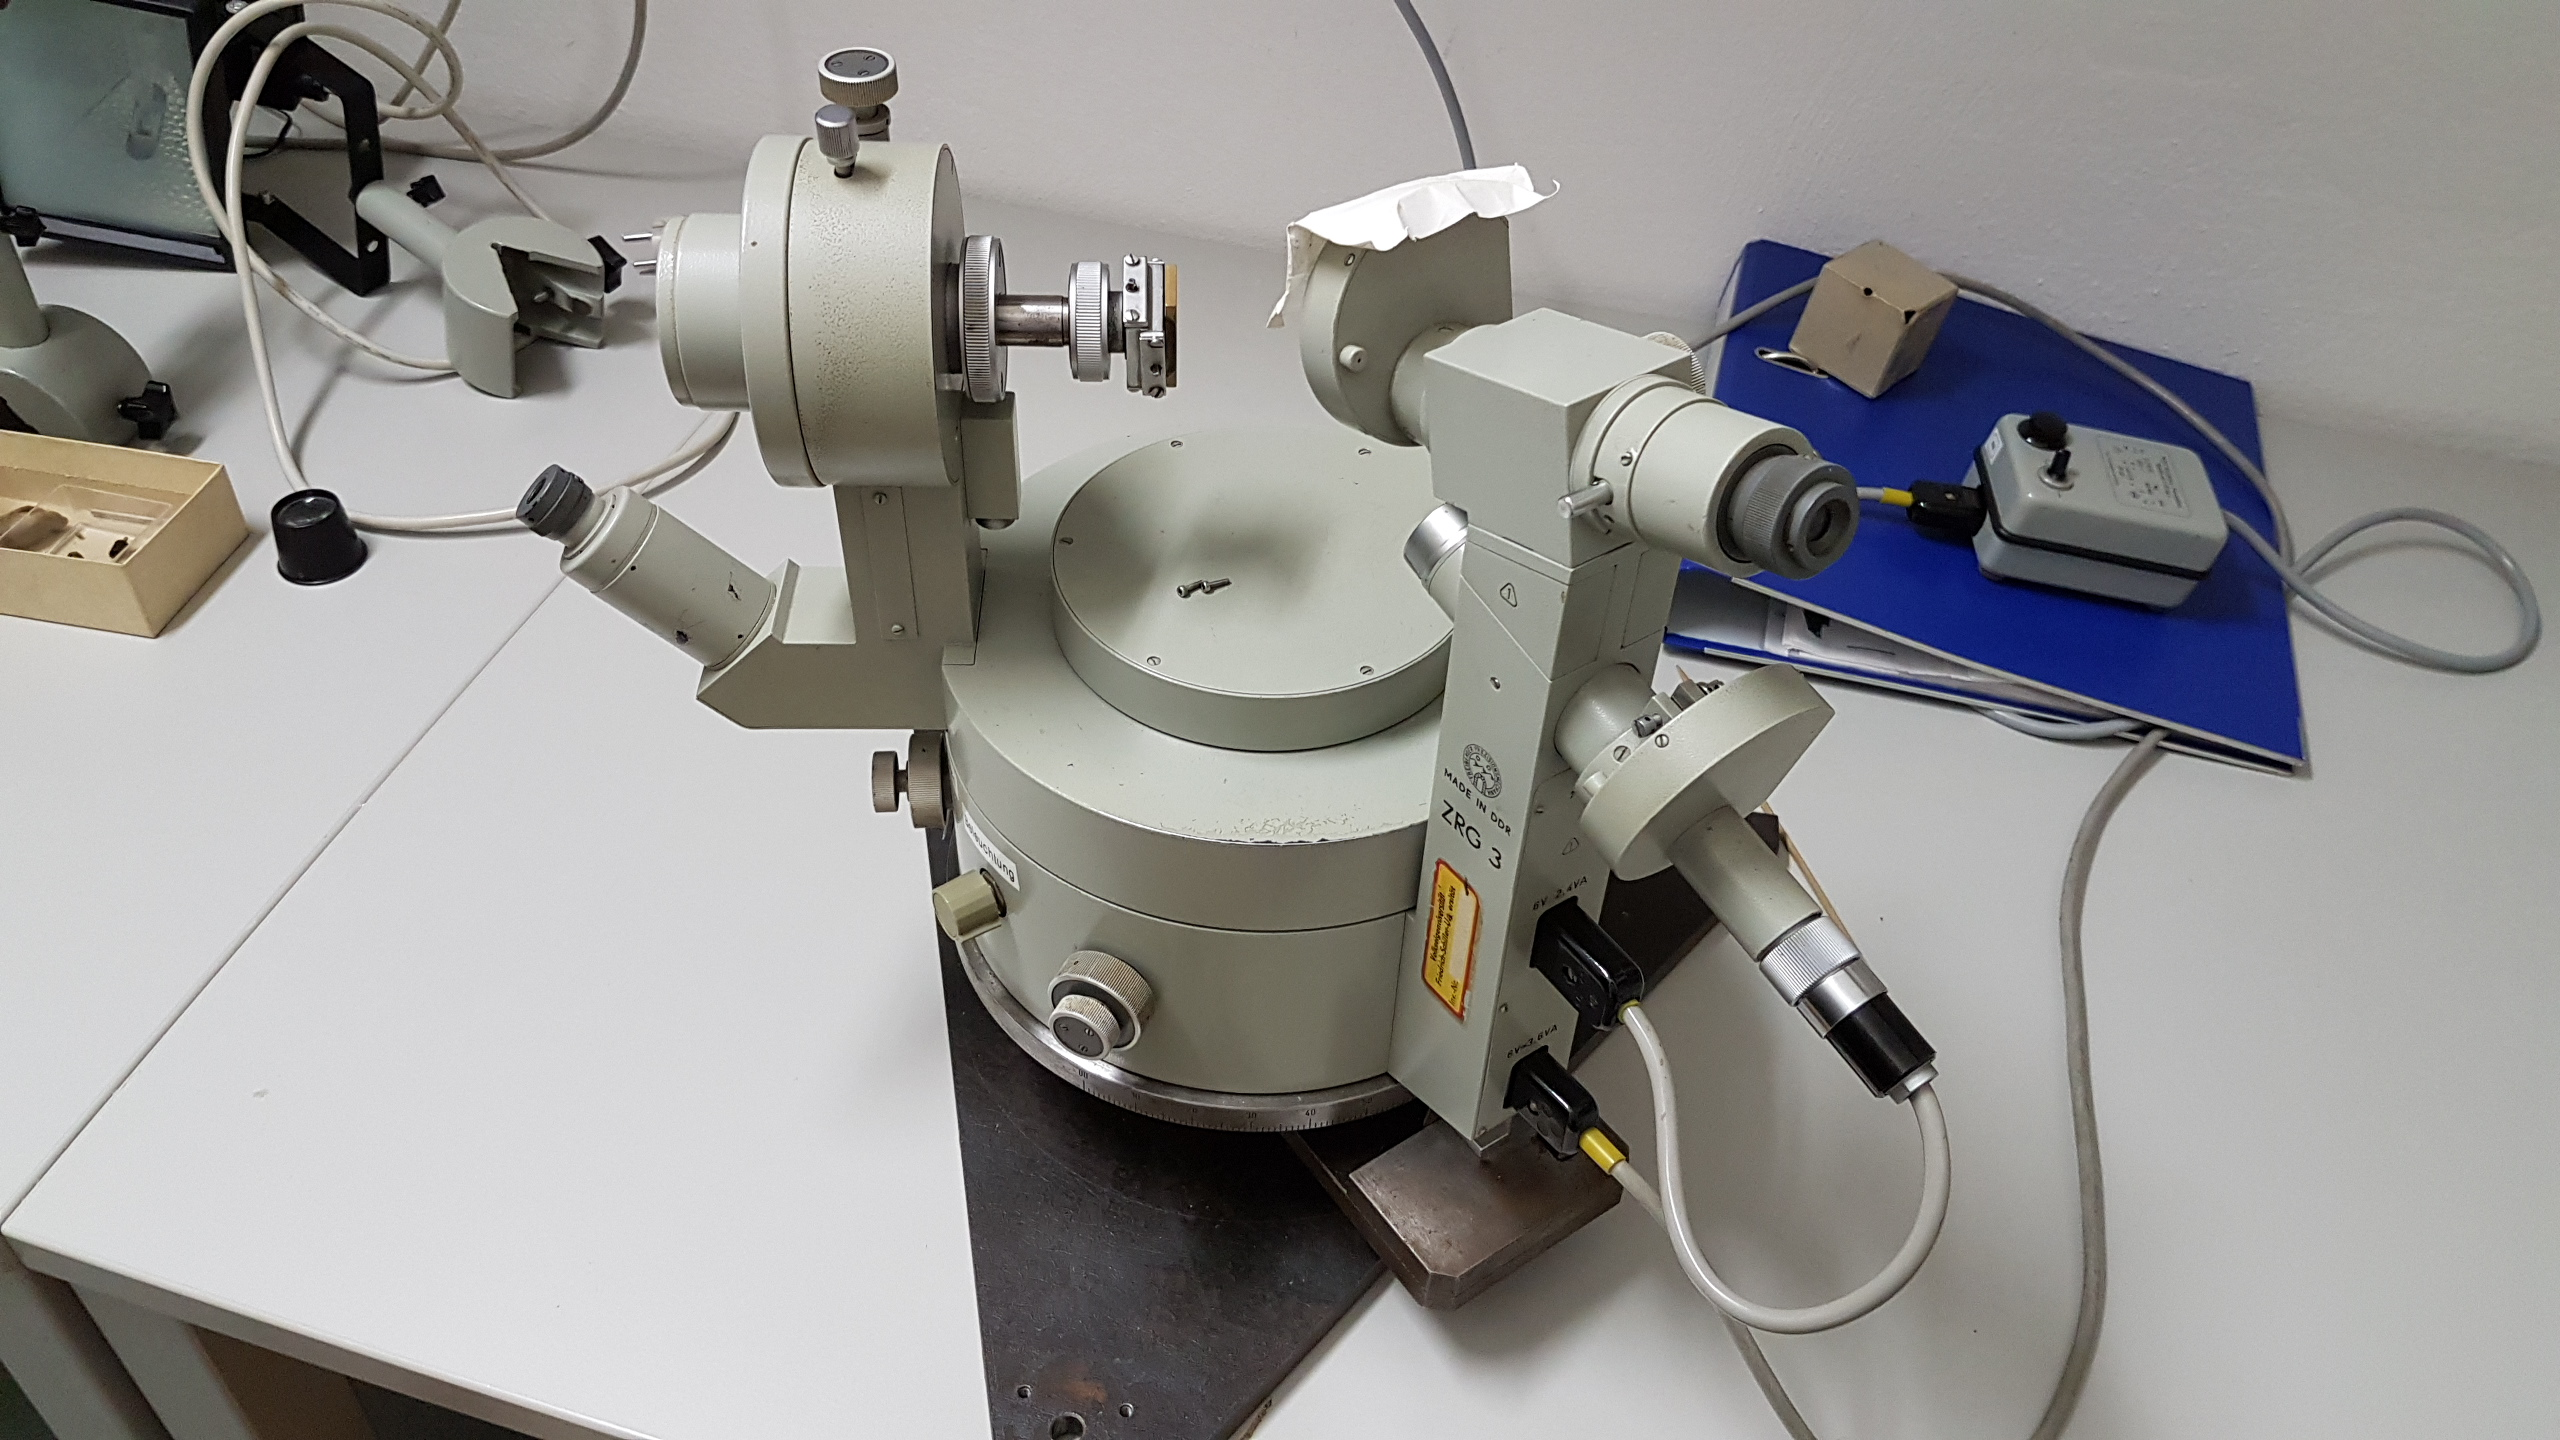
\includegraphics[scale = 0.12]{images/goniometer.jpg}
			\caption{Goniometer zur Feinjustage der Kristallachsen}
			\label{fig gonio}
		\end{figure}

	% subsection justierung_der_kristallachse (end)

% section versuchsaufbau (end)